\section{Objectives Summarised}

    \begin{enumerate}
        \item The program should be capable of procedurally drawing a road network to the UI.
        \item The number of vertices should be limited to 50 to prevent slowing down the simulation.
        \item The user should be able to save and load road networks in and out of the program.
        \item The program should support a click-and-drag based interaction, allowing the creation of vertices and connections and further editing of the network.
        \item The user should also be able to undo and redo actions to the road network.
        \item The program should be able to simulate cars driving sensibly across the road network.
        \item The maximum number of agents active at any time should be limited to 60.
        \item Relevant output data described in \autoref{analysis} should be outputted to both the UI and downloadable files.
        \item There should be a minimalist interface with the majority of screen real-estate allocated to the network visualisation.
        \item This program should support desktop size displays.
        \item It should also be compatible with variable aspect ratios, resizing UI elements to fit the screen.
    \end{enumerate}

\section{Test Descriptions}

    Each of the below tests relates to the corresponding objective shown above, I intend to show rigorously the functionality of all of these features.

    \subsection{Test 1 - Road network rendering}

        \subsubsection{Methodology}

            For this test I will demonstrate the program's ability to render road networks to the UI. I will achieve this by building a series of example networks using the built-in tools and taking screenshots of the UI.

        \subsubsection{Results}

            \begin{figure}
                \centering
                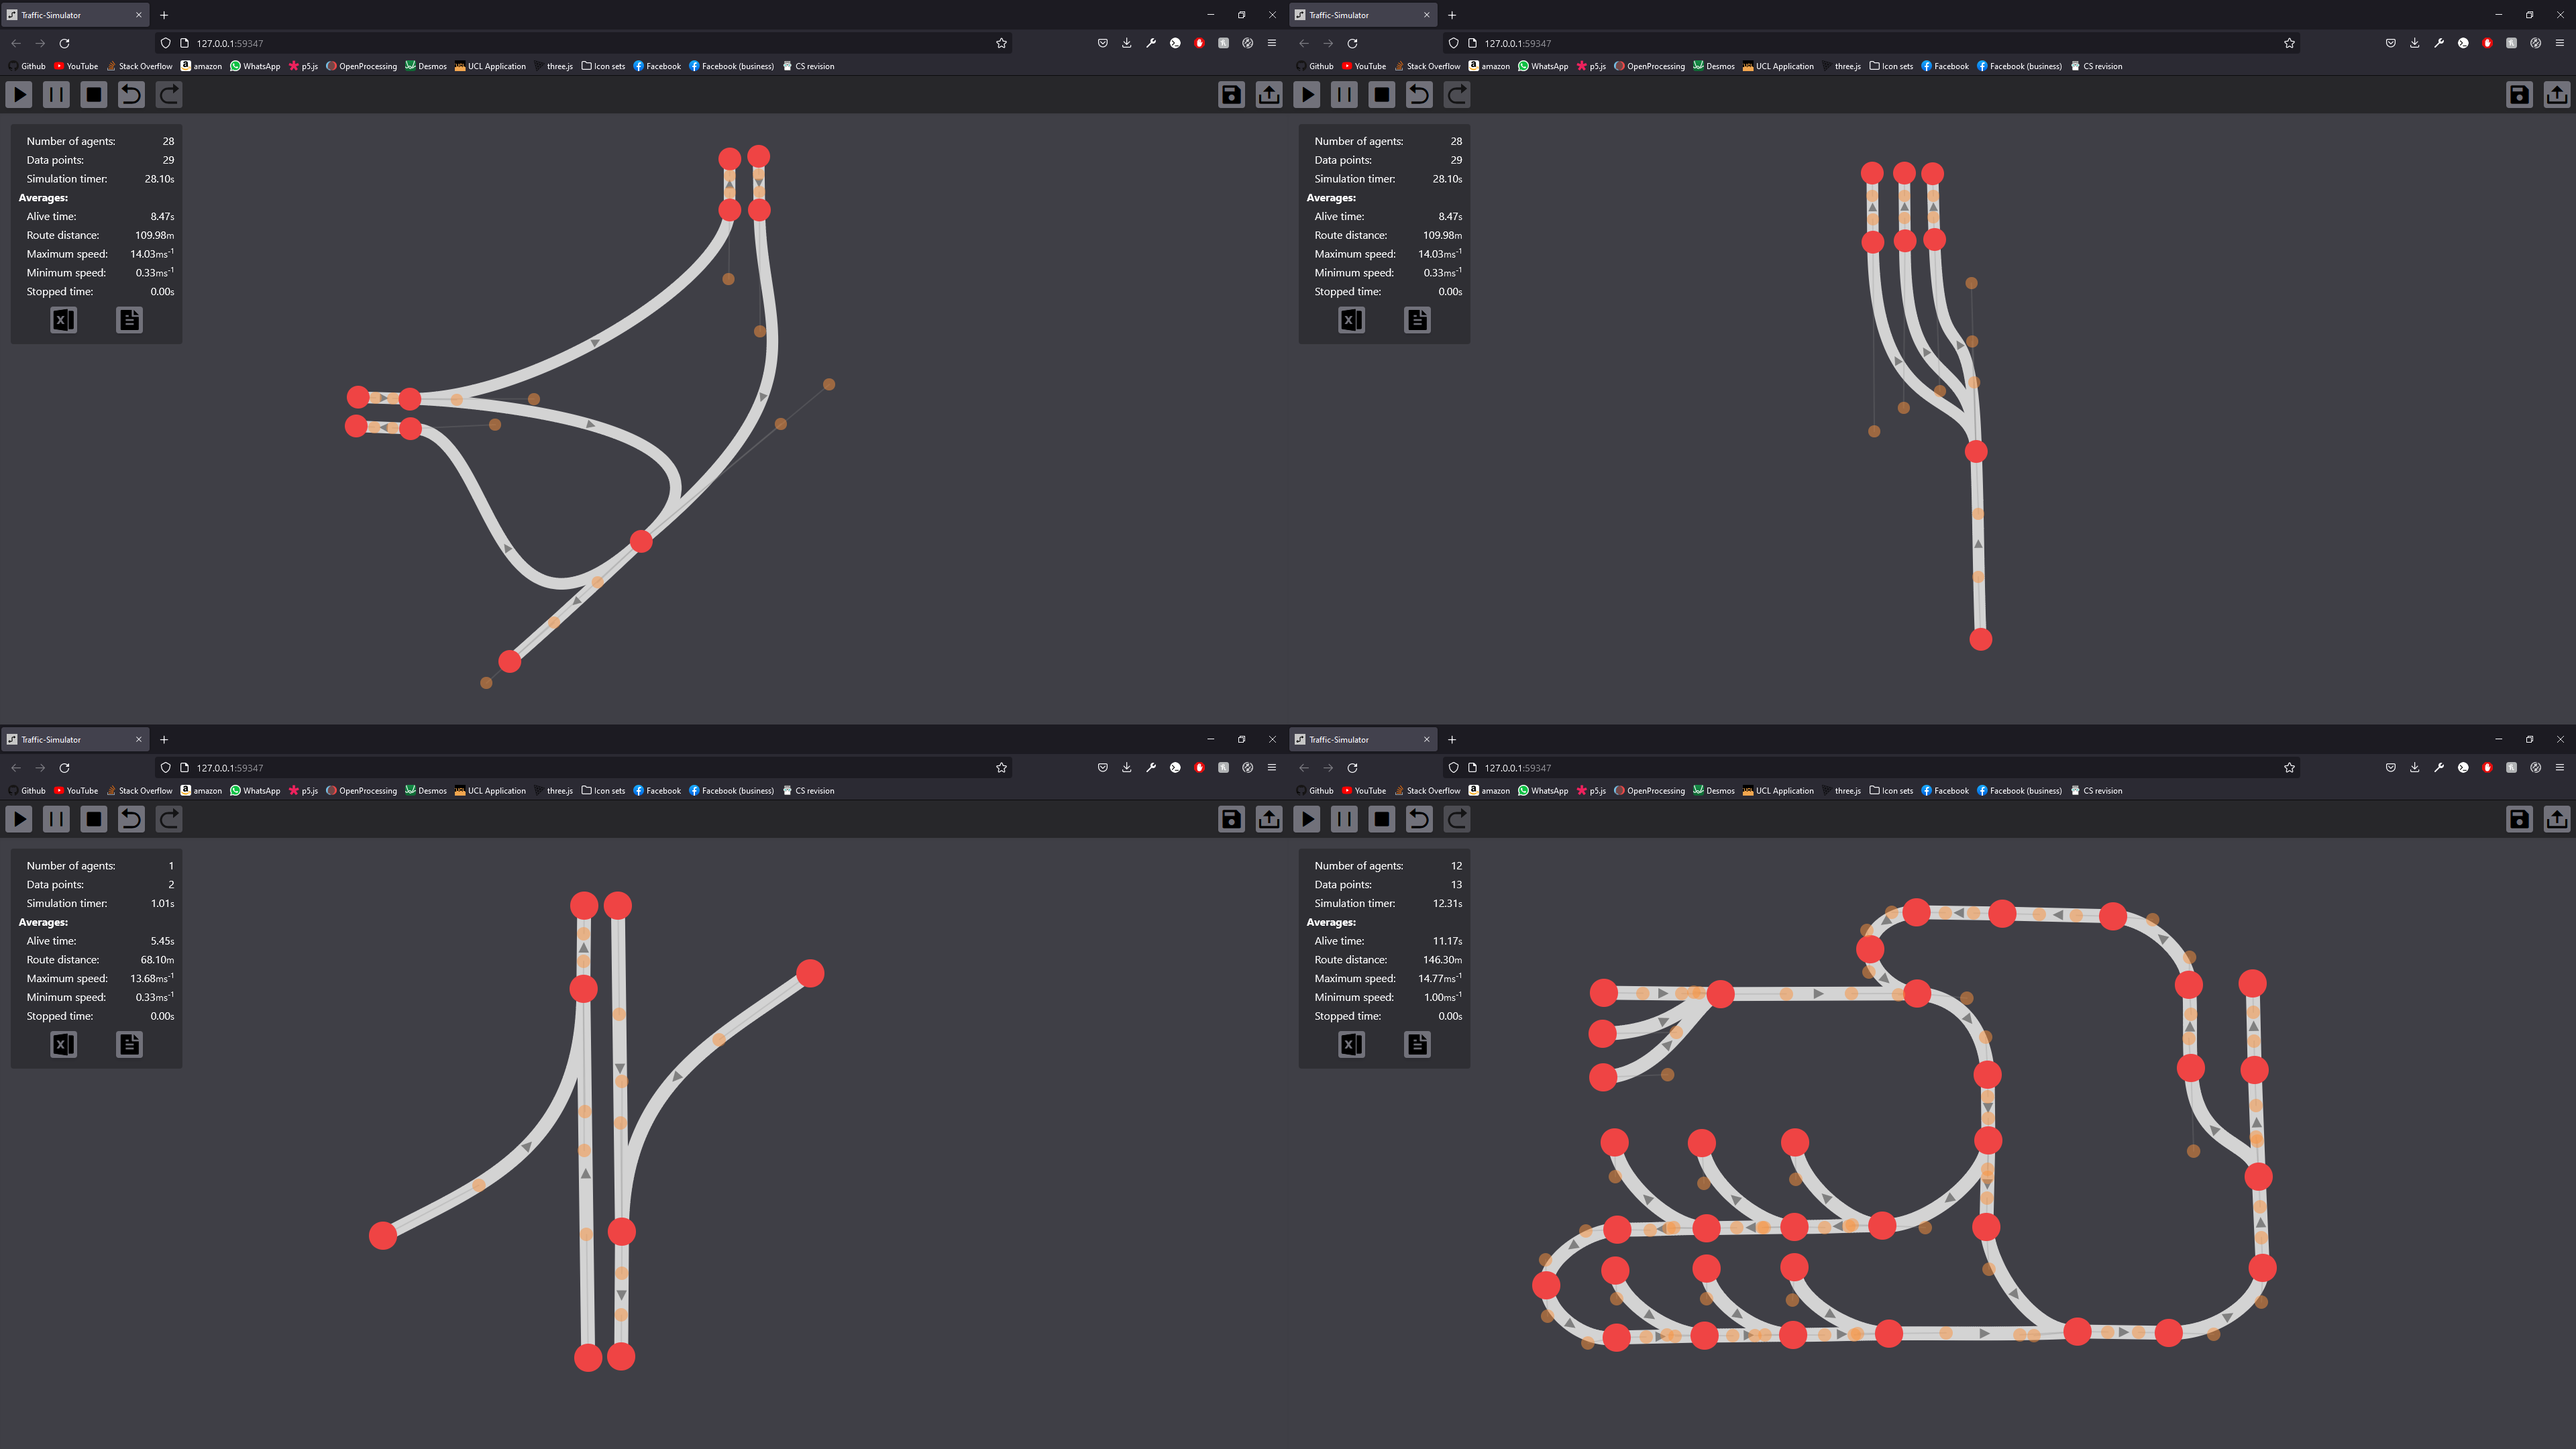
\includegraphics[width=0.8\textwidth]{example-layouts.png}
                \caption{Example road network layouts designed using my program}
                \label{testing:example-layouts}
            \end{figure}

            Shown in \autoref{testing:example-layouts} are four example layouts I constructed, all networks are rendered to the UI as expected, displaying smooth curves and everything is positioned correctly.

    \subsection{Test 2 - Vertex limit}

        \subsubsection{Methodology}

            For this test I will record a video of me using the program, I will continually create new vertices until the limit is reached. Also testing the different ways of creating new vertices to ensure that there is no way for a user to surpass the limit.

            I will also add an input overlay to the video, allowing the viewer to see the inputs I have made in real time.

        \subsubsection{Results}

            The recorded video can be found at \textbf{INSERT VIDEO LINK HERE}. The test ran as expected and the user was not able to create new vertices after the limit of 50 was reached. New connections that would have usually created a new node also behaved correctly when 50 vertices were already present.

    \subsection{Test 3 - Save and Load}

        \subsubsection{Methodology}

            \begin{enumerate}
                \item Start up the program
                \item Make a simple edit to the road network
                \item Take a screenshot of the edited network
                \item Use the save feature to save the network to a local file
                \item Take a screenshot of the file inside file explorer
                \item Take a screenshot of the file's contents
                \item Restart the program
                \item Use the load feature to load the saved network into the program
                \item Take a screenshot of the new program state
            \end{enumerate}

            The expected result of this test is to have the first an last screenshots show an identical road network. The file should also contain text formatted JSON data.

            \subsubsection{Results}

                \textbf{INSERT SCREENSHOTS HERE}

    \subsection{Test 4 - Road network construction}

        \subsubsection{Methodology}

            This test will require another video, I will start the program and use every tool provided by the program to edit the network. Theses features are as follows:

            \begin{itemize}
                \item Create new vertex
                \item Remove vertex
                \item Create new road
                \item Change road direction
                \item Remove road
                \item Create road to new vertex
                \item Reposition vertex
                \item Reposition road control point
            \end{itemize}

            I will demonstrate these features in order during the video.

        \subsubsection{Results}

            \textbf{INSERT VIDEO HERE}

    \subsection{Test 5 - Undo and Redo}

        \subsubsection{Methodology}

            \begin{enumerate}
                \item Start up the program
                \item Take a screenshot of the program state
                \item Make 2 simple edits to the road network
                \item Take another screenshot
                \item Use the undo feature to undo one action
                \item Take another screenshot
                \item Use the redo feature to redo one action
                \item Take a final screenshot of the program state
            \end{enumerate}

            The expected result of this test is to have the third screenshot show a single edit made to the original road network and the fourth to show two edits.

        \subsubsection{Results}

            \textbf{INSERT SCREENSHOTS HERE}

    \subsection{Test 6 - Agent Movement}

        \subsubsection{Methodology}

            For this test I will start the simulation using a fresh launch and making no changes to the default road network. I will capture a video of the agents moving over an arbitrary 30 second time period.

        \subsubsection{Results}

            \textbf{INSERT VIDEO HERE}

    \subsection{Test 7 - Maximum agent limit}

        \subsubsection{Methodology}

            Admittedly this feature is a little harder to test, for this test I will need to construct a rather large network, capable of holding 60 agents. I will then run the simulation and wait for 60 agents to spawn and be concurrently active in the network, when I think this point has been reached and the number of agents is no longer increasing I will take a few screenshots of the program, I will then count the number of agents on screen and verify that this number does not exceed 60.

        \subsubsection{Results}

            \textbf{INSERT IMAGE HERE}

\section{Front-end}

    \subsection{Network construction}

        As shown in \autoref{testing:gui-screenshot}, I have developed a program that displays a 2D road network. Utilising a graph data structure on the back end along with cubic Bezier curves to allow for curving road sections.

        \begin{figure}
            \centering
            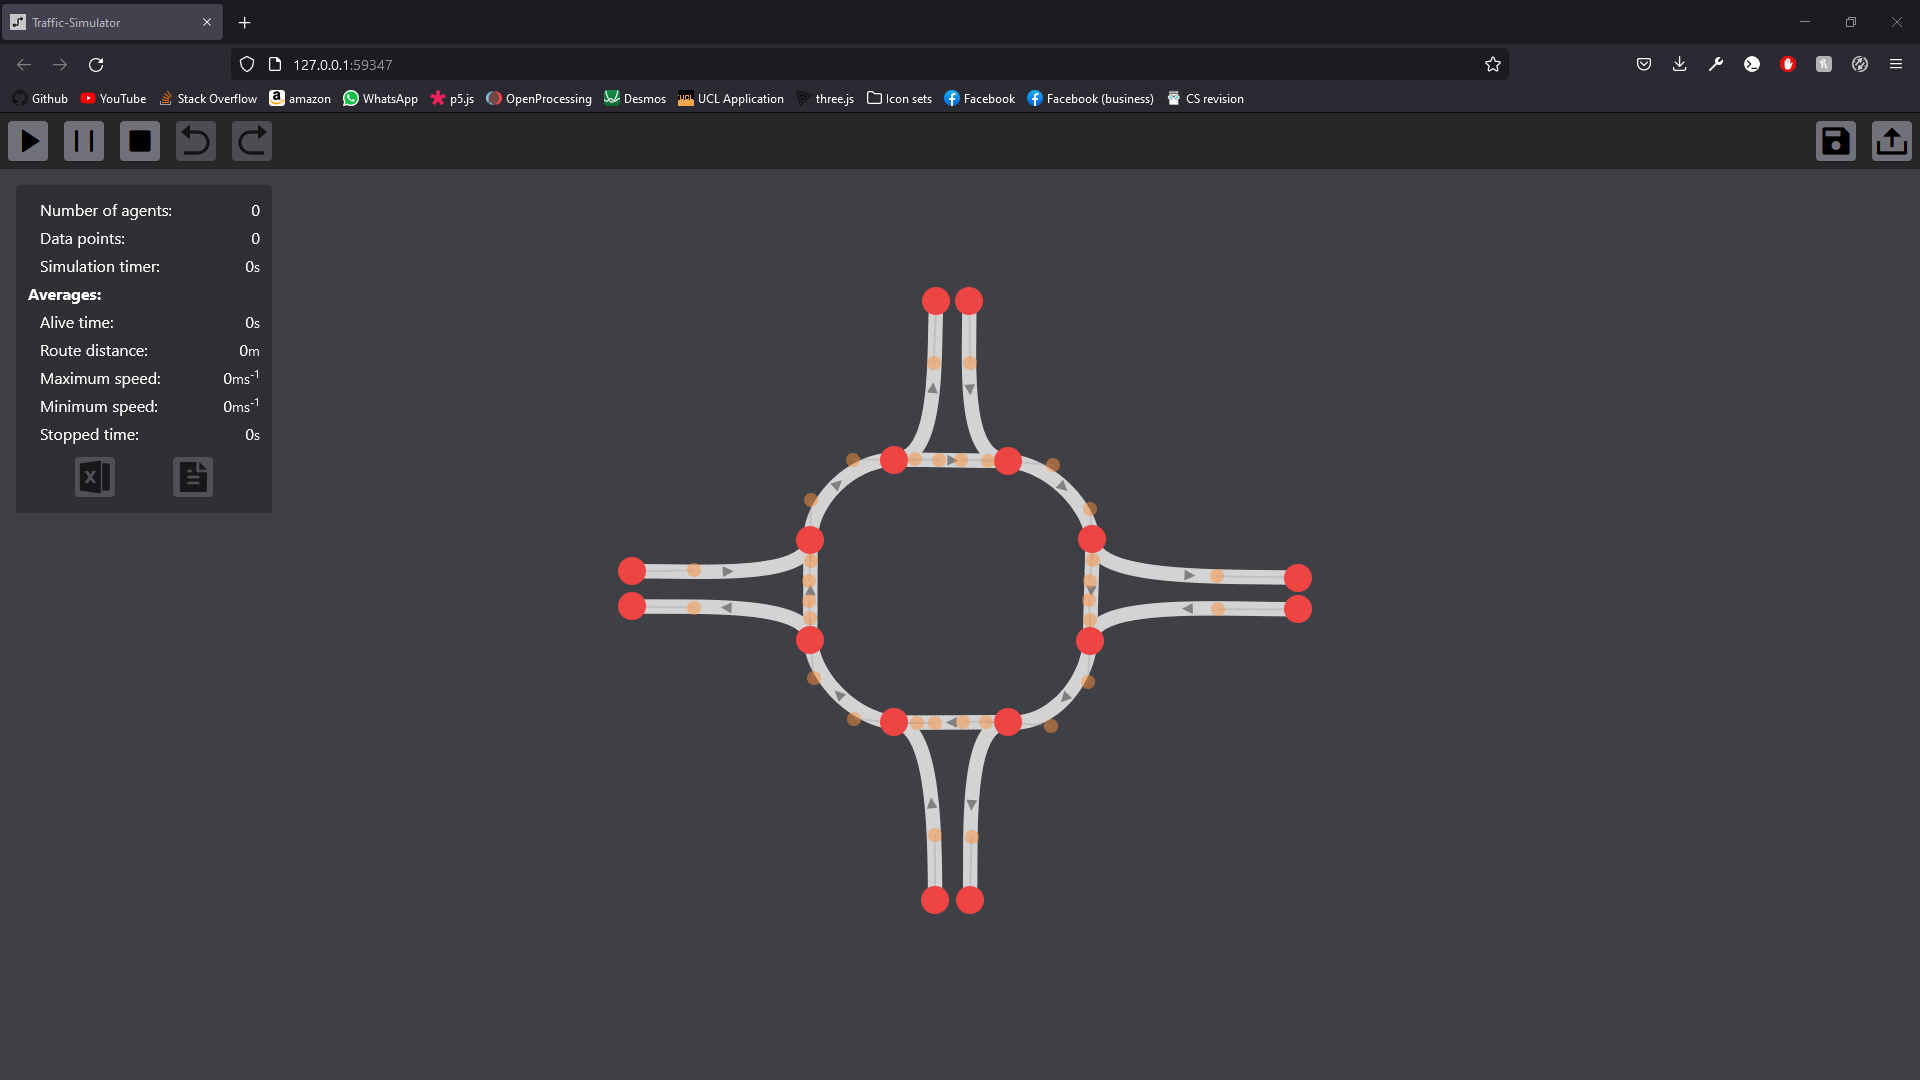
\includegraphics[width=0.6\textwidth]{gui-screenshot.png}
            \caption{Screenshot of final program}
            \label{testing:gui-screenshot}
        \end{figure}

        I have also implemented a mainly mouse-based graph editing system, allowing the user to manipulate and design their own road network. \autoref{testing:construction-examples} shows a few demo networks I have built using this program.


    \subsection{Videos}

        As part of the testing process for this project I have produced a video displaying the front-end user interaction. Making use of the majority of features I have implemented. Please note that the keyboard and mouse overlay are for clarity purposes only and not part of the program.

        \href{https://youtu.be/RnU7ZQtnQWU}{NEA testing video 1}

\section{Back-end}

    During the development process I wrote a series of unit tests to validate the major parts of the system, leading to less error-prone and maintainable code. The following index (\autoref{tests-index}) points to the test files in my code base. All the tests pass when executed.

    \begin{table}
        \begin{tabular}{|p{0.45\textwidth}|p{0.45\textwidth}|}
            \hline
            \textbf{Test target} & \textbf{Link}\\\hline
            Graph & \href{https://github.com/joshua-smart/traffic-simulator/blob/main/src/tests/model/graph.test.ts}{src/tests/model/graph.test.ts}\\\hline
            RoadNetwork & \href{https://github.com/joshua-smart/traffic-simulator/blob/main/src/tests/model/roadNetwork.test.ts}{src/tests/model/roadNetwork.test.ts}\\\hline
            Simulation & \href{https://github.com/joshua-smart/traffic-simulator/blob/main/src/tests/model/simulation.test.ts}{src/tests/model/simulation.test.ts}\\\hline
        \end{tabular}
        \caption{Unit tests index}
        \label{tests-index}
    \end{table}
